\section{Konzept}
Hier wird ein Konzept mit Mock Ups und Architektur entstehen

\subsection{Priorisierung der Erfassungsmöglichkeiten}
\subsectionauthor{Lukas Seemann}
Im Anschluss an die Auswahl der Erfassungsmöglichkeiten werden diese Möglichkeiten nun priorisiert. In der folgenden Tabelle (Tabelle 1) ist die Priosierung abgebildet. \newline
\begin{table}[h]
	\centering
	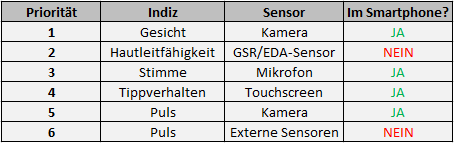
\includegraphics[width=14cm]{Bilder/prio.png}
	\caption[Priorisierung der Erfassungsmöglichkeiten]{Priorisierung der Erfassungsmöglichkeiten}
\end{table}%
\newline In der ersten Spalte ist die Priorität dargestellt. Je niedriger die Zahl ist, desto höher ist die Erfassungsmöglichkeit priorisiert. Die Möglichkeiten werden in der Reihenfolge der hier dargestellten Priorisierung thematisiert und letzten Endes in den Prototyp der mobilen Applikation integriert, um Daten zu erfassen. Je nachdem wie viel Zeit die einzelnen Features benötigen, können mehr und mehr Möglichkeiten der Datenerfassung in die App eingebaut werden, wenn sie noch im Zeitrahmen der Studienarbeit umsetzbar sind. Bei den einzelnen Möglichkeiten werden das Indiz, anhand dessen Rückschlüsse auf eine Emotion gemacht werden kann, und ein Sensor, der Daten zum Indiz für die App erfassen soll, aufgelistet. In der letzen Spalte ist festgehalten, ob der benötigte Sensor in den meisten aktuellen Smartphones bereits enthalten ist oder nicht. \newline
Die höchste Priorität hat das Indiz der Hautleitfähigkeit, die mithilfe von GSR- beziehungsweise EDA-Sensoren erfasst werden kann. Diese Art von Sensoren befinden sich nicht in handelsüblichen Smartphones, weshalb man hierzu externe Sensoren mit dem Handy verbinden muss. \newline
...

\subsection{Übertragung biometrischer Daten in Indikatorscores}
\subsectionauthor{Lukas Seemann}
Die von den Smartphone-internen und externen Sensoren zurückgeliefert Daten müssen in der App einheitlich verarbeitet werden. Die zurückgelieferten Daten sind unterschiedlich und meistens selbst nicht aussagend. Mit dem im Theorieteil erklärten Hintergrundwissen ist es jedoch möglich, die Daten zu interpretieren. Im Umfeld der App soll diese Interpretation mithilfe von Indikatoren geschehen. Ein Indikator ist in diesem Kontext ein Anzeichen, das für die Emotionsbestimmung herangezogen werden kann. Es existieren einerseits Indikatoren, die sich nur für die Bestimmung einer Emotion eignen, und andererseits auch Indikatoren, die für mehrere Emotionen ausschlaggebend sind. Folgende Indikatoren sind für die Umsetzung geplant: 
\begin{itemize}[noitemsep, topsep=0pt]
	\item stress,
	\item happyIndicator,
	\item sadIndicator,
    \item angryIndicator und
    \item suprisedIndicator.
\end{itemize}
In Abbildung ? ist der Ablauf der Bestimmung von Indikatorscores abbgebildet. Unabängig davon, welcher Sensor verwendet wird, seine Daten müssen immer auf diese Indikatoren abgebildet werden. Für jeden Sensor muss dabei ein Bereich bestimmt werden, wann immer eine neue Auswertung der Sensordaten zu den sogenannten Indikatorscores geschieht. Eine Auswertung kann generell dann durchgeführt werden, wenn genug Daten vorhanden sind, die aussagekräftig für die Indikatoren sind. Dies ist von Sensor zu Sensor unterschiedlich und muss dementsprechend berücksichitgt werden. Bei einer Auswertung werden die einzelnen Indikatoren mit Scores von null bis eins versehen, sodass man pro Auswertung der Sensordaten mehrere Indikatorscores erhält. Die Logik für das Setzen der Indikatorscores muss mithilfe von Mappern umgesetzt werden. Für jeden Sensor muss dafür ein individueller Mapper existieren. Die Mapper werden immer dann aufgerufen, wenn genügend Daten des Sensors vorhanden sind. \newline
\begin{figure}[h]
	\centering
	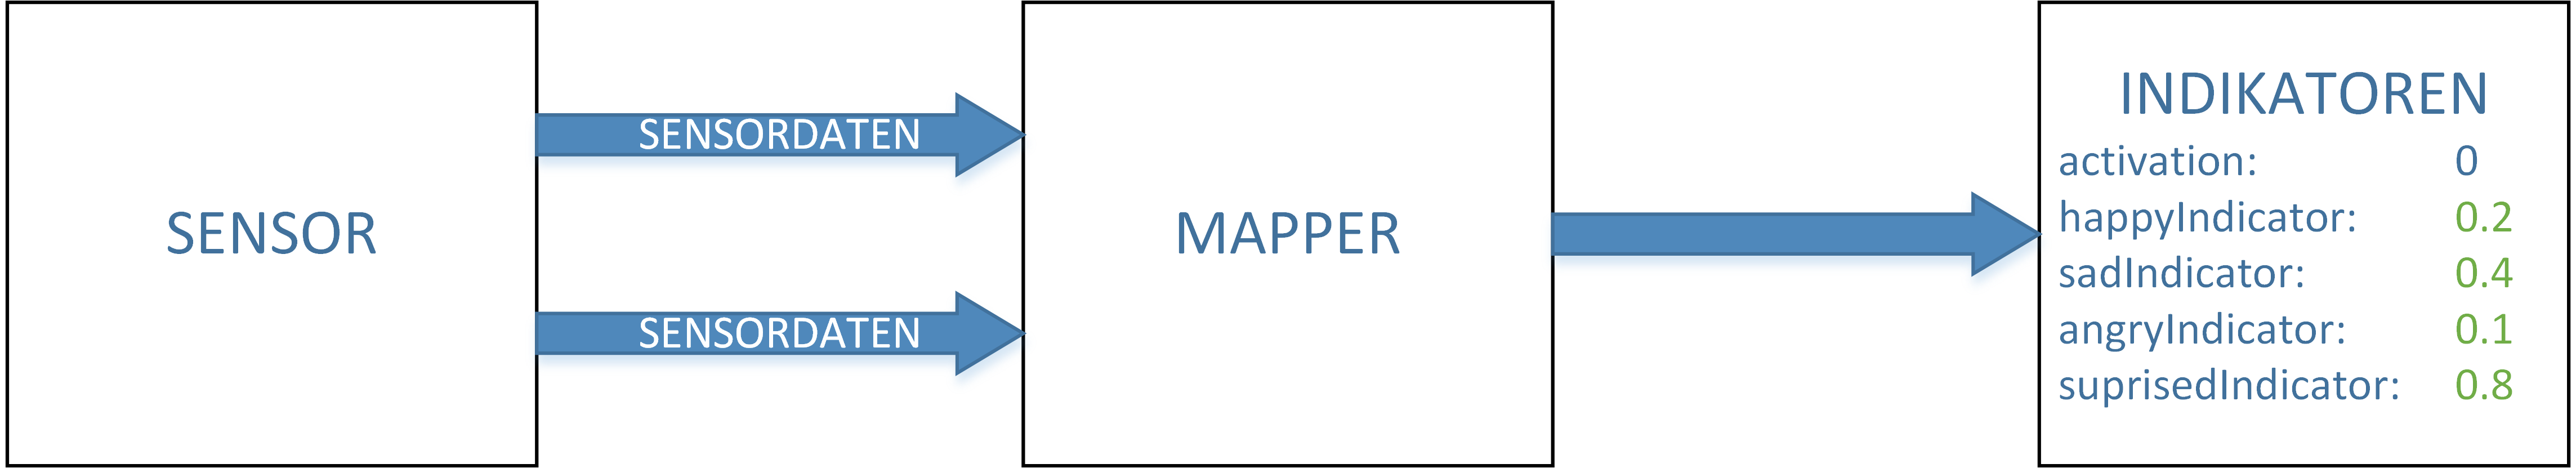
\includegraphics[width=16cm]{Bilder/indicatorscore.png}
	\caption[Ablauf der Erstellung von Indikatorscores]{Ablauf der Erstellung von Indikatorscores}
\end{figure}%
\subsection{Auswertung der Indikatorscores zur Emotionsbestimmung}
\subsectionauthor{Lukas Seemann}
Aus den angesammelten Indikatorscores muss nun entschieden werden, welche Emotion am wahrscheinlichsten beim Benutzer der App vorliegt. Diese Auswertung der Indikatorscores zu konkreten Emotionen lässt sich in zwei Bestandteile aufteilen: die Menge der Kausalitätsregeln und den Entscheidungsalgorithmus. Als Ergebnis wird pro Emotion ein Emotionscore erwartet, der angibt, inwiefern die Emotion beim User zum getesteten Zeitpunkt vorliegt.
\subsubsection{Kausalitätsregeln}
\subsubsectionauthor{Lukas Seemann}
Eine Kausalitätsregel erwartet eine Menge von Indikatorscores als Eingabe und wendet basierend auf den Indikatorscores Effekte auf die vorhandenen Emotionscores an. Die Indikatoren werden also je nach ihren Werten in verschiedene Emotionen übersetzt. Eine Kausalitätsregel besteht immer aus einer Bedingung und einer Score-Transformation. Eine Bedingung betrifft einen oder maximal zwei Indikatorscores und legt fest, wann die Score-Transformation der Kausalitätsregel ausgeführt wird. Die Score-Transformation beschreibt Effekte, die auf die Emotionscores angewandt werden. Beispielsweise würde einer hoher Score des Stress-Indikators zu positiven Effekten für die Emotionen happy, angry und suprised führen. In Abbildung ? ist der Ablauf der Ausführung einer solchen Kausalitätsregeln gezeigt. Die Formulierung von realitätsgetreuen Kausalitätsregeln ist ausschlaggebend dafür, wie präzise die Anwendung letzten Endes die Emotionen bestimmmen kann. \newline
\begin{figure}[h]
	\centering
	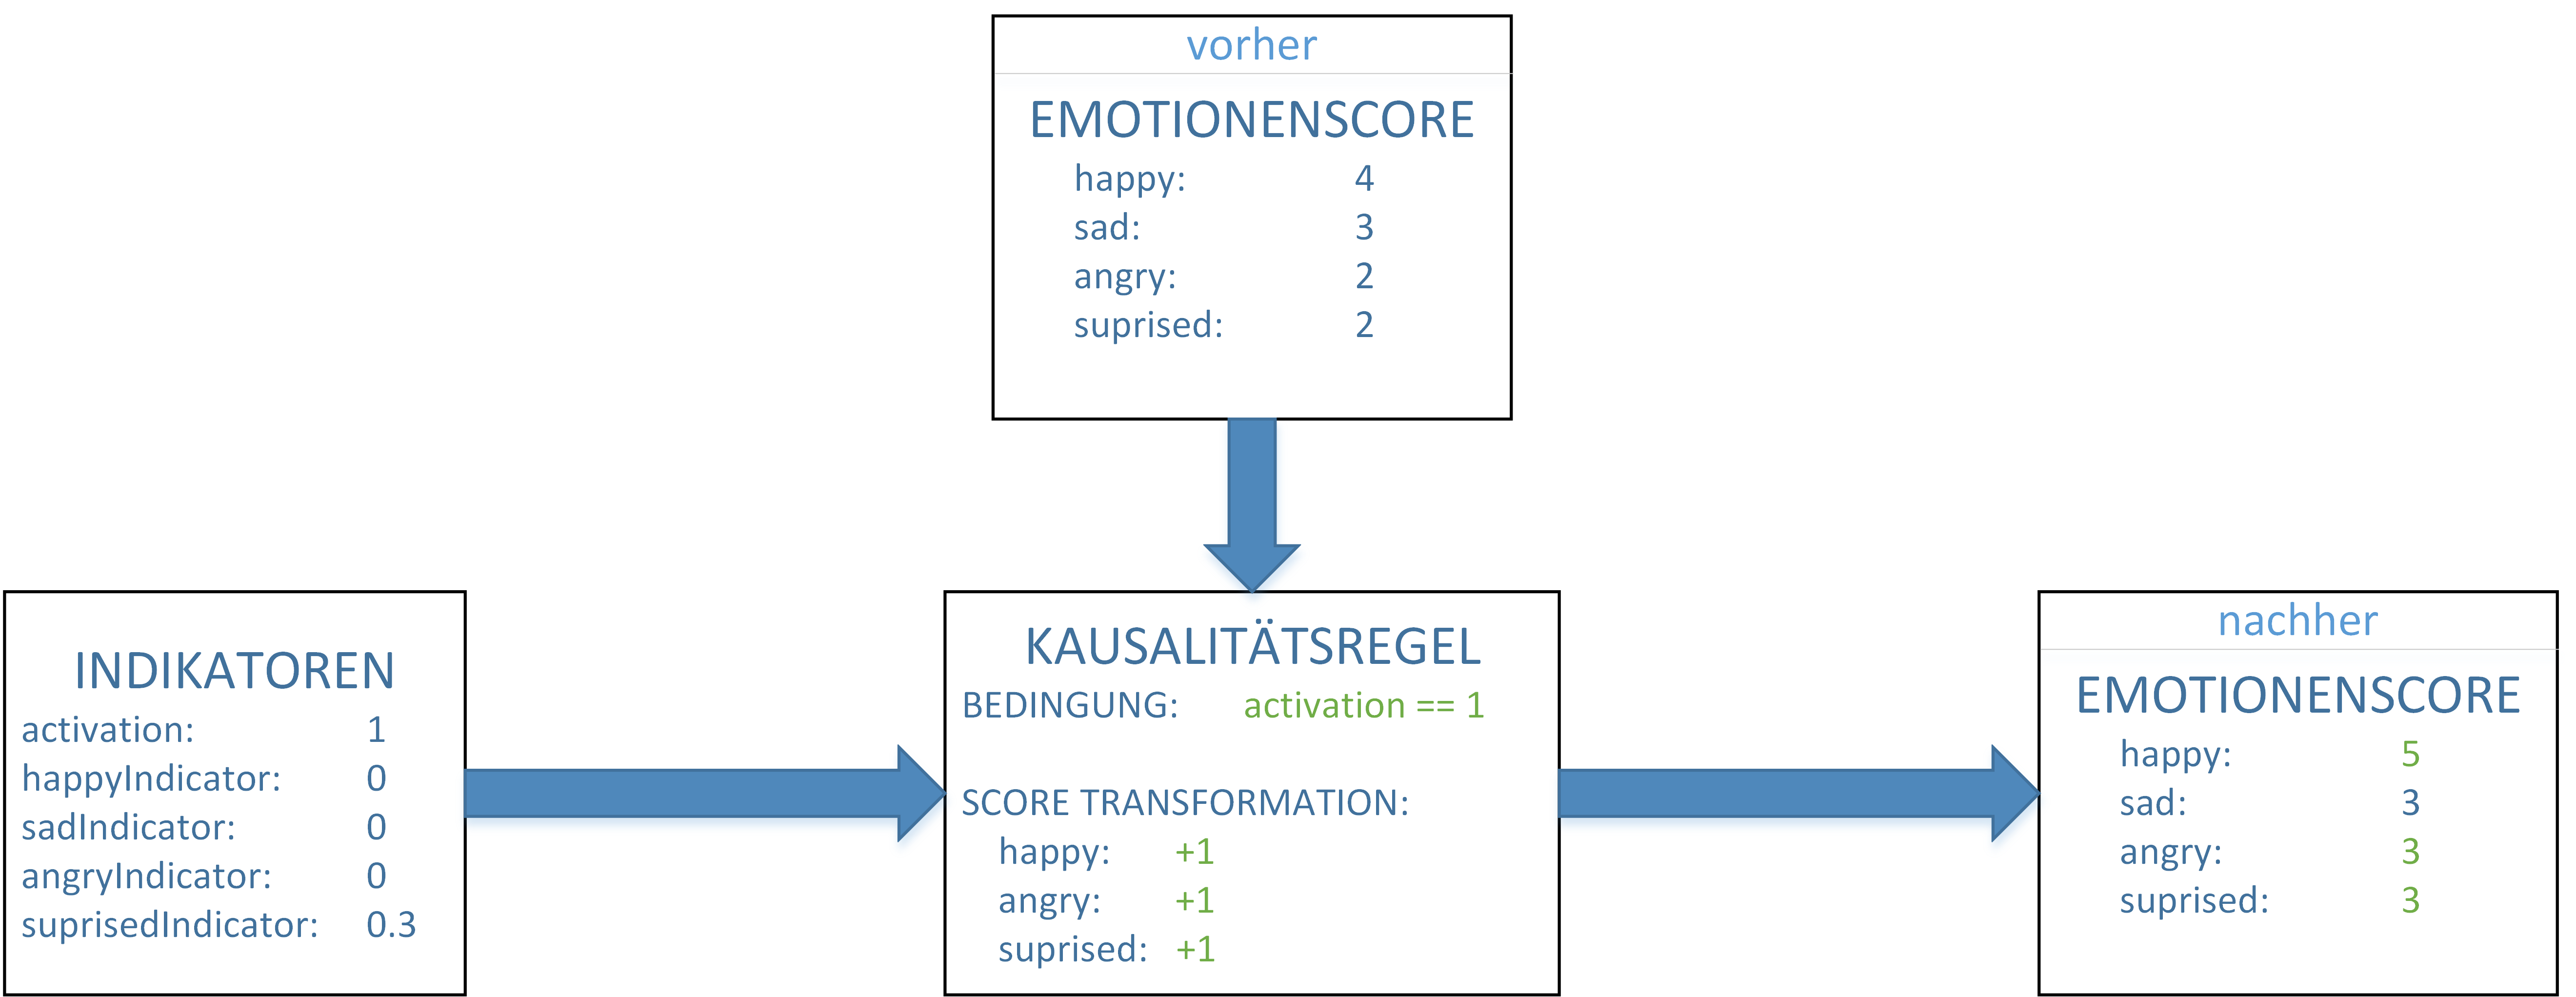
\includegraphics[width=16cm]{Bilder/causalityrules.png}
	\caption[Ablauf der Ausführung von Kausalitätsregeln]{Ablauf der Ausführung von Kausalitätsregeln}
\end{figure}%
\subsubsection{Entscheidungsalgorithmus}
\subsubsectionauthor{Torben Brenner}
Ziel der Anwendung ist es, basierend auf zuvor aufgenommenen Daten eine Entscheidung zu fällen, welche Emotion der Nutzer der 
Anwendung aktuell empfinden könnte. Die Entscheidung muss dabei die verschiedenen Ergebnisse der Auswertungsebene einbeziehen
und aus diesen auf eine Emotion schließen. Deshalb muss eine Einheitliche Datenstruktur entwickelt werden, über die die Auswertungsebene
die Daten zur Verfügung stellt. \\
Die Entscheidung könnte hierbei über ein \textit{Scoring} entstehen. Dieses \textit{Scoring} müsste dabei auf der Auswertungsebene stattfinden, 
wobei jeder der Auswertungsalgorithmen ein \textit{Scoring} für die verschiedenen Emotionen angeben muss. Am Ende könnten z. Bsp. die verschiedenen 
\textit{Scorings} addiert und die Emotion mit dem höchsten \textit{Scoring} ausgewählt werden.
\subsection{Ionic Framework}
In diesem Kapitel wird das Ionic Framework, das für die Umsetzung der mobilen Applikation verwendet wird, vorgestellt und die Gründe für die Verwendung aufgezeigt.
\subsubsection{Aufbau und Einsatz des Frameworks}
\subsubsectionauthor{Lukas Seemann}
Ionic ist ein unter der MIT License stehendes Open-Source-Framework, das zur Entwicklung von plattformübergreifenden, mobilen Applikationen dient. Mit Ionic entwickelte Apps sind damit unter anderem auf Endgeräten lauffähig, die die Betriebssysteme Android, iOS und Windows Phone benutzen. \footcite{Ion18a}
\begin{figure}[h]
	\centering
	
\includegraphics[width=11cm]{Bilder/ionic.png}
	\caption[Ionic Framework - Logo]{Ionic Framework - Logo\footnotemark}
\end{figure}%
\footcitetext{Wik18}
\newline
Aktuell befindet sich das Framework in der Version 3.9.2\footcite[Vgl. ][]{Ion18b} und befindet sich in stetiger Weiterentwicklung. Das Ionic Framework basiert wiederum auf Angular, einem Framework für die Entwicklung von Web-Applikationen. Dementsprechend nutzen Ionic-Anwendungen in der Web-Entwicklung etablierte Technologien wie HTML 5, CSS und JavaScript. \footcite[Vgl. ][]{Ion18c} Wie auch im Angular Framework, wird auch die Programmiersprache TypeScript verwendet, die auf JavaScript aufbaut, sich in der Syntax sehr stark mit JavaScript ähnelt und zusätzliche Optionen zur Typisierung von Variablen oder Funktionen anbietet. \footcite[Vgl. ][]{Til17} \newline
Ionic-Anwendungen sind im Wesentlichen normale Webanwendungen, die von jedem JavaScript-fähigen Browser ausgeführt werden können. Während mithilfe von Ionic das Frontend der Anwendung festgelegt wird, kann anschließend mit Apache Cordova die Plattformunabhängigkeit umgesetzt werden. Apache Cordova bewirkt, dass sich die Webanwendungen wie native Android-, iOS- oder Windows Phone-Applikationen anfühlen. Egal auf welcher Plattform die Ionic-Anwendung installiert wird, es wird die selbe Code-Basis verwendet. Diese wird dann vor dem Installieren von Cordova so angepasst, dass sie auf den Endgeräten ausgeführt werden können. \footcite{Ion18d}
\subsubsection{Gründe für die Verwendung}
Das Ionic Framework bietet eine Möglichkeit mit nur einer Code-Basis, eine plattform-übergreifende Applikation zu erstellen. Dies erspart einiges an Entwicklungsaufwand, da nicht jede Plattform einzeln entwickelt werden muss. Außerdem wird einem Großteil der Smartphone-Nutzer die Nutzung der erstellten App ermöglicht und ist nicht nur für Android- oder Apple-Nutzer beschränkt. \newline
Außerdem wurden bereits in anderen Projekten und im privaten Bereiche Erfahrungen mit dem Ionic Framework gemacht, sodass keine Einarbeitung bei den Entwicklungsarbeiten notwendig ist. Dies spart wiederum Zeit, die effektiv für das Entwickeln genutzt werden kann. 
\subsection{Architektur der mobilen Applikation}
